\documentclass{beamer}
\usepackage[english]{babel}
\usepackage[utf8x]{inputenc}
\usepackage{amsmath}
\usepackage{graphicx}

\title{7.2 Tangent \& normal lines (12.1 IB SL)}
\author{Dr. Huson}
\date{\today}

\begin{document}

\frame{\titlepage}

\section[Outline]{}
\frame{\tableofcontents}

\section{Drui}
\frame
{
  \frametitle{GQ: What is the tangent line's equation?}

  \begin{itemize}
  \item CCSS: Derivatives
  \item Do Now: Express $\sqrt{x}$ as a fractional exponent.\\
  Derive the derivative of $f(x)=x^3$. What is the gradient of the tangent of $f$ when $x=-2$
  \item Lesson: The derivative of $f(x)=x^n$ (p. 203)
  \item Homework:     
  \end{itemize}
}

\section{Prior learning}
\frame
{
  \frametitle{Prior learning}
  \alert{Perpendicular slopes:} The slopes of perpendicular lines are negative reciprocals.
  \[m \cdot m_{\perp} = -1\]
  \alert{Point-slope:} The equation of the line with slope $m$ through the point $(x_1,y_1)$ is 
  \[y-y_1 = m(x-x_1)\]
}

\section{Definition of a normal line}
\frame
{
  \frametitle{Definition of a normal line}
  \begin{definition}
  A \alert{normal} line is perpendicular to a given curve at a point.
  \end{definition}
  \href{https://www.geogebra.org/m/Zm97a6AJ}{link}
  \begin{figure}
    \centering
    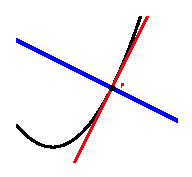
\includegraphics[height=0.4\textheight]{7-2_tangent+normal.eps}
  \end{figure}
  How would the slope of a tangent or normal line relate to $f(x)$? 
}

\section{Using the derivative for tangent and normal lines}
\frame
{
  \frametitle{Using the derivative for tangent and normal lines.\\Example 7 p205}
  \only<1-2>{What is the tangent to  $f(x)=x^2+1$ through $(1,2)$?}
  \only<2>{Steps:
  \begin{enumerate}
      \item Take derivative of the function
      \item Calculate the slope of the tangent or normal at the point
      \item Use the point-slope line formula
  \end{enumerate}}
  \only<3>{Write the equation of each line.\\[10pt]
  (a) The tangent to $f(x)=x^2+1$ through $(1,2)$\\[10pt]
  (b) The normal to $f(x)=2\sqrt{x}$ when $x=9$\\[10pt]
  (c) The tangent and normal to $\displaystyle f(x)=x+\frac{27}{2x^2}$ when $x=3$\\[10pt]
  (d) The tangent to $f(x)=x^3-3x^2-13x+15$ parallel to the tangent at $(4,-21)$}
  }

\section{Using the derivative for tangent and normal lines}
\frame
{
  \frametitle{Using the derivative for tangent and normal lines.\\Example 7d p205}
  (d) What is the equation of the tangent to \[f(x)=x^3-3x^2-13x+15\] parallel to the tangent at $(4,-21)$?
  \hspace{1in} \href{https://www.geogebra.org/m/UqZN4JgF}{link}
  \begin{figure}
    \centering
    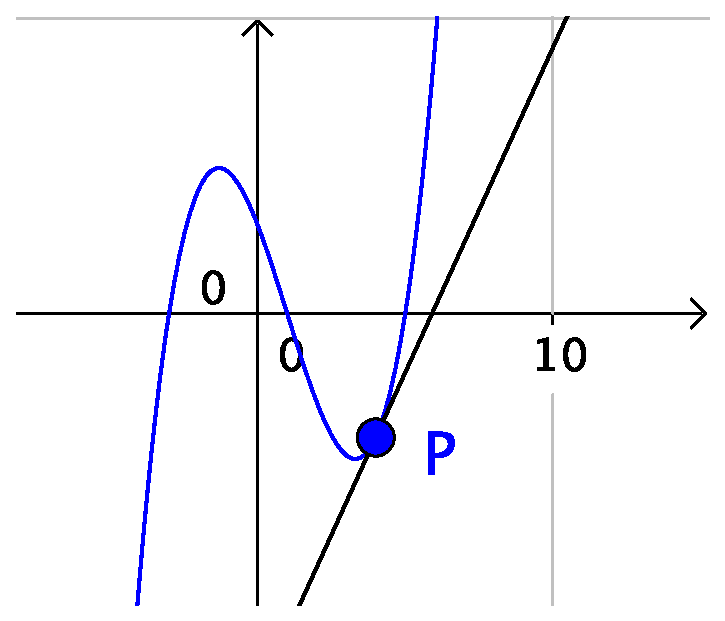
\includegraphics[height=0.4\textheight]{7-2_example7-p205.eps}
  \end{figure}
}  

\section{Exam-style questions}
\frame
{
  \frametitle{Exam-style questions. Exercise 7G, p207}
  (4) Find the equations for all the vertical normal lines to the graph of  $f(x)=x^3-3$\\[20pt]
  (5) The gradient of the tangent line to the graph of  $f(x)=2x^2+kx-3$ at $x=1$ is 1. Find the value of $k$.
  }

\end{document}